\documentclass[../mathNotesPreamble]{subfiles}
\begin{document}
%\relscale{1.4} %TODO
\section{17.4: Green's Theorem}

  \begin{thmBox*}[Green's Theorem --- Circulation Form]
    Let $C$ be a simple closed piecewise-smooth curve, oriented counterclockwise, that encloses a connected and simply connected region $R$ in the plane. Assume $\mathbf F=\bracket{f,g}$, where $f$ and $g$ have continuous first partial derivatives in $R$. Then
      \[\underbrace{\oint_C \mathbf F\cdot d\vecr}_{\textcolor{blue}{\textnormal{circulation}}}=\underbrace{\oint_C f\,dx+g\,dy}_{\textcolor{blue}{\textnormal{circulation}}}=\iint\limits_R\parens{\frac{\partial g}{\partial x}-\frac{\partial f}{\partial y}}\,dA.\]
  \end{thmBox*}

  \begin{flushright}
    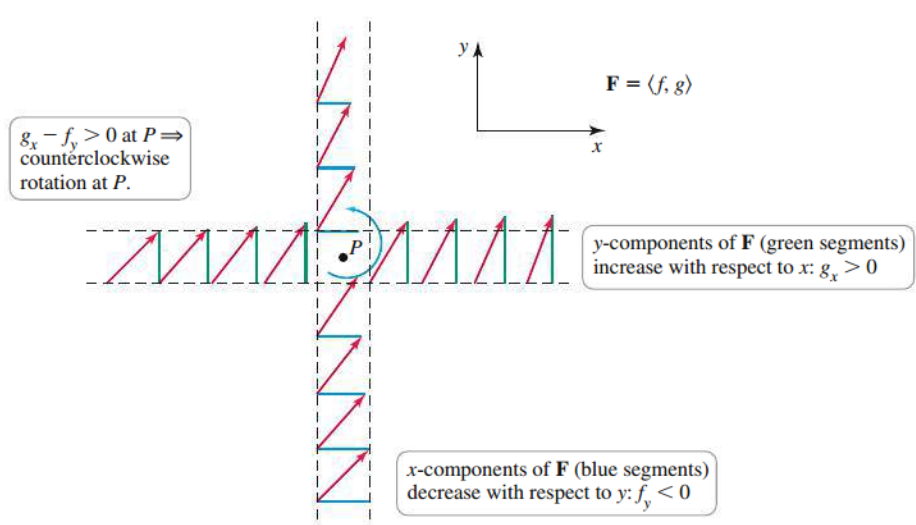
\includegraphics[width=0.825\linewidth]{../images/briggs_17_04/fig17_32}
  \end{flushright}

  \begin{defn*}[Two-Dimensional Curl]
    The \textbf{two-dimensional curl} of the vector field $\mathbf F=\bracket{f,g}$ is $\displaystyle \frac{\partial g}{\partial x}-\frac{\partial f}{\partial y}$. If the curl is zero throughout a region, the vector field is \textbf{irrotational} on the region.
  \end{defn*}
  \pagebreak

  \noindent
  \begin{ex*}
    Consider the following vector fields $\mathbf F$ over the region $R=\set{(x,y): x^2+y^2\leq 1}$. Compute the circulation using Green's Theorem.
  \end{ex*}
  
  \begin{tasks}[after-item-skip=\stretch{1}, label=](1)
    \task 
      $\mathbf F=\bracket{-y, x}$\\
      \begin{flushright}
        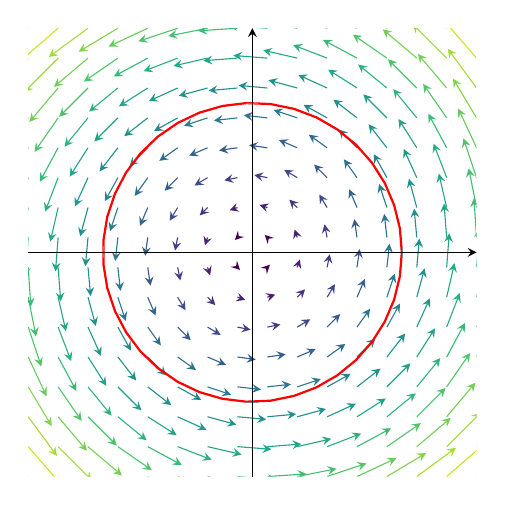
\begin{tikzpicture}
          \begin{axis}[
            	xmin = -1.5, xmax = 1.5,
            	ymin = -1.5, ymax = 1.5,
            	zmin = 0, zmax = 1,
            	axis equal image,
            	axis lines =center,
            	xtick distance = 1,
            	ytick distance = 1,
            	xticklabels={},
            	yticklabels={},
            	view = {0}{90},
            	colormap/viridis,
             ]
             \addplot3[
               point meta = {sqrt(x^2+y^2)},
               quiver = {
               u = -y,
               v = x,
               scale arrows = 0.175,
               },
               quiver/colored = {mapped color},
               samples=16,
               -stealth,
               domain = -1.5:1.5,
               domain y = -1.5:1.5,] {0};
              \draw [red, thick,  domain=0:2*pi, samples=40] 
                plot ({cos(deg(\x))}, {sin(deg(\x))} );
          \end{axis}
        \end{tikzpicture}
      \end{flushright}

    \task 
      $\mathbf F=\bracket{x, y}$\\
      \begin{flushright}
        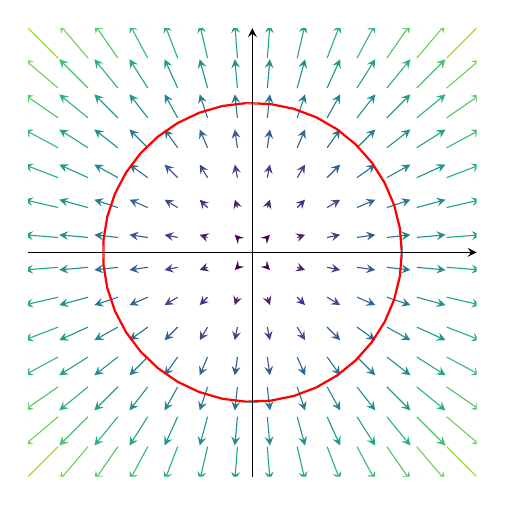
\begin{tikzpicture}
          \begin{axis}[
            	xmin = -1.5, xmax = 1.5,
            	ymin = -1.5, ymax = 1.5,
            	zmin = 0, zmax = 1,
            	axis equal image,
            	axis lines =center,
            	xtick distance = 1,
            	ytick distance = 1,
            	xticklabels={},
            	yticklabels={},
            	view = {0}{90},
            	colormap/viridis,
             ]
             \addplot3[
               point meta = {sqrt(x^2+y^2)},
               quiver = {
               u = x,
               v = y,
               scale arrows = 0.175,
               },
               quiver/colored = {mapped color},
               samples=16,
               -stealth,
               domain = -1.5:1.5,
               domain y = -1.5:1.5,] {0};
              \draw [red, thick,  domain=0:2*pi, samples=40] 
                plot ({cos(deg(\x))}, {sin(deg(\x))} );
          \end{axis}
        \end{tikzpicture}
      \end{flushright}
  \end{tasks}
  \vspace*{\stretch{1}}
  \pagebreak

  \begin{ex*}
    Compute the curl of $\mathbf F=\bracket{x^2,2y^2}$ where $C$ is the upper half of the unit circle and the line segment $-1\leq x\leq 1$.
  \end{ex*}
  \vspace*{\stretch{0.5}}

  \begin{thmBox*}[Area of a Plane Region by Line Integrals]
    Under the conditions of Green's Theorem, the area of a region $R$ enclosed by a curve $C$ is
      \[\oint_C x\,dy=-\oint_C y\,dx=\frac{1}{2}\oint_C\parens{x\,dy-y\,dx}.\]
  \end{thmBox*}

  \begin{ex*}
    Find the area of the ellipse $\displaystyle \frac{x^2}{a^2}+\frac{y^2}{b^2}=1$.
  \end{ex*}
  \vspace*{\stretch{1}}
  \pagebreak

  \begin{thmBox*}[Green's Theorem --- Flux Form]
    Let $C$ be a simple closed piecewise-smooth curve, oriented counterclockwise, that encloses a connected and simply connected region $R$ in the plane. Assume $\mathbf F=\bracket{f,g}$, where $f$ and $g$ have continuous first partial derivatives in $R$. Then
      \[\underbrace{\oint_C \mathbf F\cdot \vecn\, ds}_{\textcolor{blue}{\textnormal{outward flux}}}=\underbrace{\oint_C f\,dy-g\,dx}_{\textcolor{blue}{\textnormal{outward flux}}}=\iint\limits_R\parens{\frac{\partial f}{\partial x}+\frac{\partial g}{\partial y}}\,dA,\]
    where $\vecn$ is the outward unit normal vector on the curve.
  \end{thmBox*}

  \begin{flushright}
    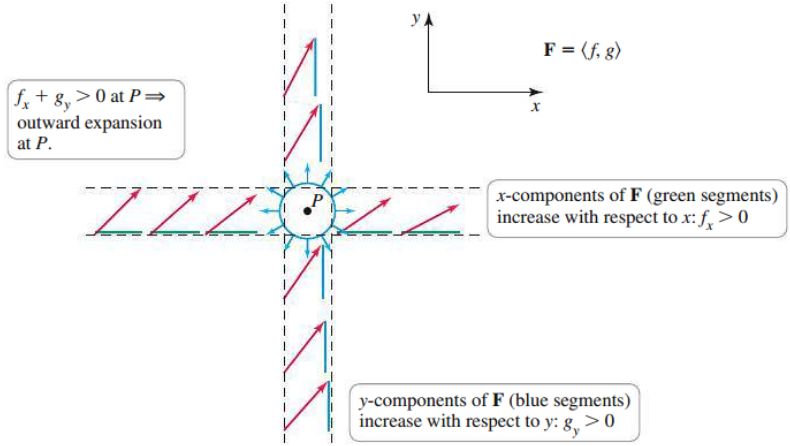
\includegraphics[width=0.9\linewidth]{../images/briggs_17_04/fig17_33}
  \end{flushright}

  \begin{defn*}[Two-Dimensional Divergence]
    The \textbf{two-dimensional divergence} of the vector field $\mathbf F=\bracket{f,g}$ is $\displaystyle \frac{\partial f}{\partial x}+\frac{\partial g}{\partial y}$. If the divergence is zero throughout a region, the vector field is \textbf{source free} on that region.
  \end{defn*}
  \pagebreak

  %% \begin{ex*}
  %%   Evaluate
  %%     \[\oint_C \parens{4x^3+\sin(y^2)}\,dy-\parens{4y^3+\cos(x^2)}\,dx\]
  %% \end{ex*}
  %% \vspace*{\stretch{1}}
  %% \pagebreak

  \begin{ex*}
    Integrate $\displaystyle \oint_C \parens{2x+e^{y^2}}\,dy-\parens{4y^2+e^{x^2}}\,dx$, where $C$ is the boundary of the square with vertices $(0,0)$, $(1,0)$, $(1,1)$, and $(0,1)$.
  \end{ex*}
  \vspace*{\stretch{1}}
  \pagebreak

  \begin{ex*}
    Compute the circulation and outward flux across the boundary of the given regions:
  \end{ex*}
  \begin{tasks}[after-item-skip=\stretch{1}, label=](1)
    \task $\mathbf F=\bracket{x,y}$; $R$ is the half-annulus $\set{(r,\theta): 1\leq r\leq 2, 0\leq \theta\leq \pi}$,
  \end{tasks}
  \vspace*{\stretch{1}}
  \pagebreak

  \begin{tasks}[after-item-skip=\stretch{1}, label=, resume](1)
    \task $\mathbf F=\bracket{-y,x}$; $R$ is the annulus $\set{(r,\theta): 1\leq r\leq 3, 0\leq \theta\leq 2\pi}$.
  \end{tasks}
  \vspace*{\stretch{1}}
  \pagebreak

  \textbf{Stream functions:}\newline
  In the same way that a vector field is conservative if there exists a potential function $\varphi$, a vector field is source free if a \textbf{stream function} $\psi$ exists such that
    \[\frac{\partial \psi}{\partial y}=f, \hspace*{25pt} \frac{\partial \psi}{\partial x}=-g.\]
  If such a function exists, then the divergence is zero:
    \[\frac{\partial f}{\partial x}+\frac{\partial g}{\partial y}=\underbrace{\frac{\partial}{\partial x}\parens{\frac{\partial \psi}{\partial y}}+\frac{\partial}{\partial y}\parens{-\frac{\partial \psi}{\partial x}}}_{\textcolor{blue}{\displaystyle\psi_{yx}=\psi_{xy}}}=0\]

  If a vector field is both conservative and source-free, then it has both a potential function and a stream function. Furthermore, the level curves of the potential and stream functions form orthogonal families. These vector fields have zero divergence
    \[0=f_x+g_y=\varphi_{xx}+\varphi_{yy},\]
  and zero curl
    \[0=g_x-f_y=-\psi_{xx}-\psi_{yy}.\]
  Thus, conservative, source-free vector fields satisfy \textbf{Laplace's equation}:
    \[\varphi_{xx}+\varphi_{yy}=0 \qquad \textnormal{ and } \qquad \psi_{xx}+\psi_{yy}=0.\]
  \pagebreak

  \begin{ex*}
    For $\mathbf F=\bracket{-e^{-x}\sin(y),\,e^{-x}\cos(y)}$
  \end{ex*}
  \begin{tasks}[after-item-skip=\stretch{1}, label=](1)
    \task 
      Show $\mathbf F$ is conservative and source-free field
    \task 
      Find the potential function $\varphi$ and the stream function $\psi$
  \end{tasks}
  \vspace*{\stretch{1}}
  \pagebreak

  \begin{center}
    \renewcommand{\arraystretch}{2.5}
    \begin{tabularx}{0.95\linewidth}{@{}X@{\hspace*{60pt}}X@{}}
      \textbf{Conservative Fields $\mathbf F=\bracket{f,g}$}& \textbf{Source-Free Fields $\mathbf F=\bracket{f,g}$}\\\midrule
      %
      curl $\ds = \frac{\partial g}{\partial x}-\frac{\partial f}{\partial y}=0$& 
      divergence $\ds = \frac{\partial f}{\partial x}+\frac{\partial g}{\partial y}=0$\\
      %
      Potential function $\varphi$ with \newline
      $\mathbf F=\grad\varphi$\hfill or\hfill $\ds f=\frac{\partial \varphi}{\partial x}$,\hfill $\ds g=\frac{\partial \varphi}{\partial y}$& 
      Stream function $\psi$ with 

      $\ds f=\frac{\partial \psi}{\partial y}$, \hspace*{25pt} $\ds g=-\frac{\partial \psi}{\partial x}$\\
      %
      Circulation $\ds=\oint_C \mathbf F\cdot d\vecr=0$ on all
      
      closed curves $C$.& 
      Flux $\ds=\oint_C \mathbf F\cdot\vecn\,ds=0$ on all closed curves $C$.\\
      %
      Evaluation of the line integral \newline$\displaystyle \int_C \mathbf F\cdot d\vecr = \varphi(B)-\varphi(A)$&
      Evaluation of the line integral \newline$\displaystyle \int_C \mathbf F\cdot \vecn\,ds = \psi(B)-\psi(A)$\\\bottomrule
    \end{tabularx}
  \end{center}
  \pagebreak

  \begin{center}
    \renewcommand{\arraystretch}{1.75}
    \begin{tabularx}{\linewidth}{@{}
      >{\hsize=0.8\hsize}X
      >{\hsize=1.1\hsize}X
      >{\hsize=1.1\hsize}X@{}}\toprule
      \multicolumn{3}{c}{\textbf{Circulation/work integrals: $\displaystyle\int_C \mathbf F\cdot\vecT\,ds=\int_C\mathbf F\cdot d\vecr=\int_C f\,dx+g\,dy$}}\\\midrule
      & $C$ \textbf{closed}& $C$ \textbf{not closed}\\
      %
      $\mathbf F$ \textbf{conservative}\newline ($\mathbf F=\grad\varphi$)& $\displaystyle \oint_C \mathbf F\cdot d\vecr=0$&
      $\displaystyle \int_C \mathbf F\cdot d\vecr=\varphi(B)-\varphi(A)$\\
      %
      $\mathbf F$ \textbf{not conservative}&
      Green's Theorem\newline $\displaystyle \oint_C \mathbf F\cdot d\vecr=\iint\limits_R \parens{g_x-f_y}\,dA$&
      Direct evaluation\newline $\displaystyle \int_C\mathbf F\cdot d\vecr=\int_a^b \parens{fx'+gy'}\,dt$\\\midrule
      \multicolumn{3}{c}{\textbf{Flux integrals: $\displaystyle\int_C \mathbf F\cdot\vecn\,ds=\int_C f\,dy-g\,dx$}}\\\midrule
      & $C$ \textbf{closed}& $C$ \textbf{not closed}\\
      %
      $\mathbf F$ \textbf{source free}\newline ($f=\psi_y, g=-\psi_x$)& $\displaystyle \oint_C \mathbf F\cdot \vecn\,ds=0$&
      $\displaystyle \int_C \mathbf F\cdot \vecn\,ds=\psi(B)-\psi(A)$\\
      %
      $\mathbf F$ \textbf{not source free}&
      Green's Theorem\newline $\displaystyle \oint_C \mathbf F\cdot \vecn\,ds=\iint\limits_R \parens{f_x+g_y}\,dA$&
      Direct evaluation\newline $\displaystyle \int_C\mathbf F\cdot \vecn\,ds=\int_a^b \parens{fy'-gx'}\,dt$\\\bottomrule
    \end{tabularx}
  \end{center}
  \pagebreak

  \begin{ex*}
    Suppose $C$ is a circle centered at the origin, oriented counterclockwise, that encloses disk $R$ in the plane. For $\mathbf F=\bracket{4x^3y, xy^2+x^4}$
  \end{ex*}
  \begin{tasks}[after-item-skip=\stretch{1}, label=\alph*)](1)
    \task 
      Calculate the two-dimensional curl of $\mathbf F$
    \task 
      Calculate the two-dimensional divergence of $\mathbf F$
    \task 
      Is $\mathbf F$ irrotational on $R$?
    \task 
      Is $\mathbf F$ source free on $R$?
  \end{tasks}
  \vspace*{\stretch{1}}
  \pagebreak

  \begin{proof}
    Consider the regions $R$ enclosed by a simple closed smooth curve $C$ oriented in a counterclockwise direction, given by
      \[R=\set{(x,y): a\leq x\leq b, G_1(x)\leq y\leq G_2(x)}\]
    or
      \[R=\set{(x,y): H_1(y)\leq x\leq H_2(y), c\leq y\leq d}.\]
    \begin{center}
      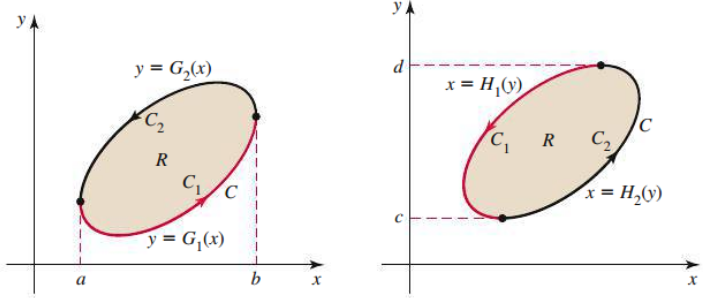
\includegraphics[width=0.65\linewidth]{../images/briggs_17_04/fig17_37}
    \end{center}
    To prove the circulation form of Green's Theorem, we have

    \begin{minipage}{0.5\linewidth}
      \begin{align*}
        &\iint\limits_R \frac{\partial f}{\partial y}\,dA\\
          &= \int_a^b \int_{G_1(x)}^{G_2(x)}\frac{\partial f}{\partial y}\,dy\,dx\\
          &=\int_a^b \big(\underbrace{f\parens{x,G_2(x)}}_{\textnormal{on }C_2}-\underbrace{f\parens{x,G_1(x)}}_{\textnormal{on }C_1}\big)\,dx\\
          &=\int_{-C_2} f\,dx-\int_{C_1} f\,dx\\
          &=-\int_{C_2} f\,dx-\int_{C_1} f\,dx\\
          &=-\oint_C f\,dx
      \end{align*}
    \end{minipage}%
    \begin{minipage}{0.5\linewidth}
      \begin{align*}
        &\iint\limits_R \frac{\partial g}{\partial x}\,dA\\
          &= \int_c^d \int_{H_1(y)}^{H_2(y)}\frac{\partial g}{\partial x}\,dx\,dy\\
          &=\int_c^d \big(\underbrace{g\parens{H_2(y),y}}_{C_2}-\underbrace{f\parens{H_1(y),y}}_{-C_1}\big)\,dy\\
          &=\int_{C_2} g\,dy-\int_{-C_1} g\,dy\\
          &=\int_{C_2} g\,dy+\int_{C_1} g\,dy\\
          &=\oint_C g\,dy
      \end{align*}
    \end{minipage}%
    
  \end{proof}
  \pagebreak 
 
\end{document}
